\chapter{Background}

% SIDDATA (mit Educational Resources dabei, muss kein sub-chapter sein)
% Conceptual Spaces (What is this?)
% Required techniques and algorithms

\section{Replication and Software Quality}

Having established the goals of replicating an algorithm for a new domain, let us look at how such a replication should be performed and how software quality can be measured.

\subsection{Replication and Reproducibility}
\label{sec:howtoreplicate}

The workflow of data science generally follows the same pattern: A paper states there is some problem \textit{X}, claims that their algorithm \textit{Y} may be good at problem \textit{X}, creates datasets \textit{Z} for \textit{X}, and then tests the code on these datasets. This test generally compares \textit{X} to alternative approaches from the literature and explores if any regularities in the algorithm \textit{Y} can be found. This may yield future research opportunities, showing what other domains the algorithm may work for as well.

Replication fills this role by applying an existing algorithm to another domain. Results for this are important, as it helps to see first if the claimed results are valid, and if they work on datasets that are not artificial and specifically created for the sole purpose of testing the algorithm. Furthermore, the details of experiments in publsihed work are often opaque and omit important information to reproduce the algorithm. These issues are mitigated trough repetition: The robustness of the algorithm to changes in parameters or dataset is investigated. If changes in either of these have a major impact on the results, there is reason to doubt generalization of the algorithm, showing that it may not be good to solve problem \textit{X} after all.

It is absolutely crucial in science to ensure that all claims that are made are reproducible and testable, ensuring ease of replication. Reproducibility is the pinnacle of \textit{Open Science}.\footnote{There is no single definition of open science, however reproducibility appears in most tries, such as \eg \url{https://www.talyarkoni.org/blog/2019/07/13/i-hate-open-science/}, accessed at \date{2022}{03}{25}} And \q{Open Science is just science done right}.\footnote{Quote from John Tennant, see \eg \url{https://soundcloud.com/tidningen-curie/jon-tennant-open-science-is-just-science-done-right}, accessed at \date{2022}{03}{25}} Reproducibility refers to the Ability to reproduce - computationally or experimentally - the methods used to produce a given result, by virtue of being accessible and understandable. Being a hot topic in psychology since the reproducibility crisis,\footnote{Baker M: 1,500 scientists lift the lid on reproducibility. Nature. 2016; 533(7604): 452-4. \url{https://www.nature.com/articles/533452a}} the topic is just es relevant in computer science research.\footnote{Mesirov JP: Computer science. Accessible reproducible research. Science. 2010; 327(5964): 415-6. \url{https://www.ncbi.nlm.nih.gov/pmc/articles/PMC3878063/}} In that realm, Reproducibility may be seen as sub-goal of (the more fundamental) Sustainability, as \eg by \textcite{Molder2021a}, who claim that \q{reproducibility alone is not enough to sustain the hours of work that scientists invest in crafting data analyses}.

To ensure that the analysis performed in this thesis is sustainable and adheres to best scientific and software quality standards, let us look at at ways to formally define such.

\subsection{Software Quality}
\label{sec:reproducibility}

The International Organization for Standardization (ISO) provides an official international standard for the evaluation of software quality as \textbf{ISO/IEC 25010:2011} \cite{2013ISOI}. The full title of the norm is \textit{ISO/IEC 25010:2011 Systems and software engineering - Systems and software Quality Requirements and Evaluation (SQuaRE)}. It has the objective to ensure the quality of software by providing objective and clearly defined standards for definitions of success regarding of software products. It classifies software quality in eight characteristics, which each consists of several sub-characteristics. The main characteristics are \textit{Functional Suitability, Performance Efficiency, Compatibility, Usability, Reliability, Security, Maintainability} and \textit{Portability}. Not all of these are relevant to projects like this, such as \textit{Security}, which mostly measures the ability to track actions and identity of users. 

What is needed here are those goals relevant for sustainable data analysis. In this realm, the stated metrics align much with the hierarchy of aspects to consider for sustainable data analysis as published by \textcite{Molder2021a}, which is is reprinted as \autoref{fig:snakemake_aspect_hierachy}.

\begin{figure}[H]
	\centering
	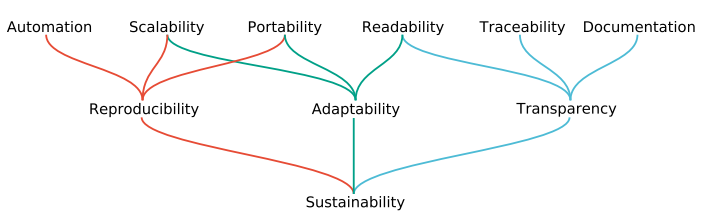
\includegraphics[width=0.7\textwidth]{graphics/stolenfigures/snakemake_aspect_hierachy.png}
	\slcaption{
		Hierarchy of aspects to consider for sustainable data analysis. Reproduced from {\cite[Fig.1]{Molder2021a}} (Creative Commons Attribution License) \label{fig:snakemake_aspect_hierachy}
	}
\end{figure}

Some important aspects to conduct proper computer science and data analysis that allows for \textbf{Sustainability} - allowing the analysis to be of lasting impact - thus include \cite{Molder2021a, 2013ISOI}:

\begin{description}
    \item[Functional Suitability] which means complete, correct and appropriate functionality.
	\item[Reproducibility] \ie allowing validation and regeneration of results on the original or even new data. This understandable and well documented code (also \textit{Changeability and Stability})
	\item[Maintainability and Adaptability] the ability to modify the analysis to answer extended or slightly different research questions by allowing modifications.
	\item[Transparency] \ie the ability for others to understand it well enough to judge if it's technically as well as methodologically valid - also ensuring Understandability, Appropriateness and Accessibility, Analyzability and Testability.
	\item[Scalability] \ie enabling the scalable execution of the algorithm and each involved step, including deployment on complex compute clusters, grids or clouds. This includes Performance Efficiency and efficient Resource Utilization.
	\item[Modularity] \ie changes in one component have a minimal impact on others allowing for easy exchange and extension.
\end{description}


% \begin{description}
%     \item[Functional Suitability], assessing the existance of a set of functions that satisfy the stated needs. It includes \textit{Functional Completeness, Functional Appropriateness (Suitability)} \textit{and Functional Correctness (Accuracy)}
%     \item[Performance Efficiency], assessing the relationship between the performance and the amount of resources used, specifially \textit{Time behaviour, Resource Utilization} and \textit{Capacity}
%     \item[Compatibility], consisting of \textit{Co-Existence and Interoperability}
%     \item[Usability], assessing the effort needed for use, measured by \textit{Appropriateness Recognizability (Understandability), Learnability, Operability, User Error Protection, Accessibility} and \textit{Interface Aesthetics (Attractiveness)}
%     \item[Reliability], assessing the capacity of software to maintain its level of performance, comprising \textit{Maturity, Fault tolerance, Recoverability} and \textit{Availability}
%     \item[Security], among others allowing to track actions and identity: \textit{confidentiality, integrity, non-repudiation, accountability} and authenticity
%     \item[Maintainability], assessing the effort needed to make modifications, which includes \textit{Analyzability, Testability, Modularity} (meaning changes in one component have a minimal impact on others), \textit{reusability} and \textit{modifiability (Changeability+Stability)}
%     \item[Portability], measruing the ability to be transferred to other environments: \textit{Adaptability, Installability} and \textit{Replaceability}
% \end{description}

% Some important aspects to conduct proper (computer) science and data analysis that allows for \textbf{Sustainability} (such that the analysis is of lasting impact), may thus be \cite{Molder2021}:
% \begin{description}
% 	\item[Reproducibility] \ie allowing validation and regeneration of results on the original or even new data. Requiring understandable and well documented code.
% 	\item[Adaptability] \ie the ability to modify the analysis to answer extended or slightly different research questions.
% 	\item[Transparency] \ie the ability for others to understand it well enough to judge if it's technically as well as methodologically valid.
% 	\item[Scalability] \ie enabling the scalable execution of the algorithm and each involved step, including deployment on complex compute clusters, grids or clouds. 
% \end{description}

% Principles of open science are very important to me, so I want to ensure that the claims I am making in this thesis are backed by code that is scalable, reproducible, modular, easily-understood, easily set up and run, well documented, ... . To support this, I will as often as necessary refer to the actual code in this thesis, to allow to understand and reproduce the claims and results, and also highly encourage to critically read everything here and check the respective code (...and let me know if you spot any errors! Just open a Github Issue!)



\section{SIDDATA and Educational Resources}
\label{sec:siddata}

\todoparagraph{Educational resources has no definition, aber siddata ist ein beispiel projekt was darum revolviert}

"Frage war ja, Lässt sich der Algo auf die Domäne von Ed.Res. beziehen, und dafür muss ich sie erklären"

\todoparagraph{auf die kategorien in} \ref{tab:siddata_metadata} hinaus: in principle könnnen educaitonal resources können auch transkribierte videos sein, PDFs als vorlesungsmaterial, ganze paper oder bücher, oder multimedia-data such as in a mooc). \todoparagraph{Hier ider in dataset-section}


% \includeMD{pandoc_generated_latex/2_0_siddata}

To get a better understanding of the domain, this section elaborates on the specific use case of recommendation of education resources that shall be handled, and introduces the SIDDATA project and platform under which this thesis was developed.\footnote{As \textsc{Siddata} signifies both the project and the developed digital assistant, the all-upper 'SIDDATA' henceforth refers to the project, while the specific developed software will be denoted 'Siddata' or 'DSA'.}

This thesis was started while working at the SIDDATA project, with the idea to add a recommender to the platform that can generate course recommendations with the user \textit{in the loop}. SIDDATA is a joint interdisciplinary project for \q{\emph{Individualization of Studies through Digital, Data-Driven Assistants}}\footnote{\url{https://www.siddata.de/en/}} of the universities Osnabrück, Bremen and Leibniz Universität Hannover, funded by the German \emph{Federal Ministry of Education and Research}.\footnote{BMBF. Funding number: 16DHB2124} 

The project adresses the same problem as stated in the Introduction (\ref{sec:many_resources}), namely that e-learning and the amount of avilable resources increase, making the choice of right resources an increasingly relevant problem for the learning success of students. Its deliverable is a flexible data-driven \gls{dsa}, that supports students in higher education in their invidual learning and achievement of personal study goals by giving hints, reminders and recommendation for their individual study paths \cite{Schurz2021}, helping students in setting and achiving individual and self-regulated personal educational goals. This is in line with the increasing importance of skills such as self-organized knowledge acquisition and self-regulatory competencies due increasing importance of individualization in educational paths of the globalized learning environment \cite{Ehlers2019,Schurz2021}.

For that, the collaborative project combines heterogenous data and information in a digital study assistant. Data is collected from multiple sources, such as the \gls{lms}, offers and resources of other universities and institutions, and data collected from its users. To allow for this heterogeniety and also future extensions, for example new data sources  such as \glspl{mooc} through several apis APIs, different front-ends, or different recommendation methods, the system relies on a highly modular and extensible architecture. The Frontend is realized as plugin for the  the university's \gls{lms} Stud.IP \cite{stockmann2005}. This not only allows for easy user access, but also to get data about courses from the LMS using cronjobs. The Frontend is connected over a RESTful API to the Backend, which is written in Python on basis of the Web Framework \textit{Django} and relies on a relational \textit{PostgreSQL} database to store information.

The Backend consists of seperate encapsulated recommender modules in a loosely coupled architecture and a common ontology, allowing to easily add new subsystems. The modules generate recommendations towards personal educational goals on basis of the collected data, which are displayed to the user in the Frontend. What comprises a recommender is grouped from a user perspective, such that each each recommender focuses on a topic. The currently implemented recommenders include for example one to find peers with similar interests, get information about scientific careers, personality-based learning behaviour- and study tips, or information regarding local and remote courses and \glspl{oer}. Another module recommends courses using a combination of rule-based and modern \gls{ml} techniques that relate natural language queries with the courses known to the system (picked up in \autoref{sec:sidbert}) \cite{Schurz2021}.

The system is currently in its third prototype, and preliminary evaluation has shown that modules that provide personal recommendation are most well received \cite{Schurz2021}. This and the ease of use to add new recommenders indicate a high likelyhood of success for adding a new module that recommends courses in the way as described above.

The dataset used here was collected through the Siddata platform as well, which collected courses and events from the three universities currently connected to it, as well as other sources for \glspl{mooc} and other \glspl{oer} through respective APIs. More details in \autoref{sec:dataset_siddata}. It should be noted that the dataset is not artificially generated (unlike \mainalgos) but collected from current courses and their descriptions - making an algorithm for this domain incorporated as recommender to the platform a contribution with practical application.



\section{Conceptual Spaces}

This section will introduce conceptual spaces as tool of choice as well as how to generate them and how reasoning on them works, as well as some other related work to what's done in this thesis.

\subsection*{Theory of Conceptual Spaces}

The theory of Conceptual Spaces was first introduced by Peter Gärdenfors in his 2000 book \citetitle{Gardenfors2000a} \cite{Gardenfors2000a} both as a theoretical model of human concept formation, but also as format for knowledge representation in artificial systems \cite{Gardenfors2004}. 

On the one hand, \glspl{cs} should serve as bridge between symbolistic and connectionistic approaches to knowledge representation. By having CS as layer of reasoning and representation in between both, classical symbols would be grounded in noisy high-dimensional data, allowing for high-level syllogistic reasoning from real-world data. 

If a computer has a knowledge base that says $\exists x.Red(x) \& Apple(x)$, does it know what "red" and "apple" mean? We need to ground symbols, to express meaning!

According to Gärdenfors, concept-representation in humans is represented by three levels of accounting for observations: The symbolic level, the conceptual level and the subconceptual level \cite[204]{Gardenfors2000a}:
\begin{description}
    \item[Subconceptual] Observations are the firing of the neurons of our sensory receptors, without any conceptualization.  (connectionism, \glspl{ann})
    \item[Conceptual] Observations are defined not as token of a symbol, but as vector in a conceptual space of some quality  (prototype theory, linear algebra)
    \item[Symbolic] represents observations by describing them in some specified language (formal logic, syllogisms, symbolism, classical AI, logical positivism)
\end{description}

These levels are not in conflict, but different models of the same phenonemon, each covering distinct important aspects and each allowing a set of algorithms. The process of inducing a general rule from few samples for example is represented as pattern-matching on the firing patterns in the subconceptual level, which translates to the conceptual level as geometric reasoning through regions and direction. As another example, semantic relations such as hyponyms from the symbolic level are modelled as geometric sub-regions on the conceptual level. So on the one hand, automatically generated conceptual spaces could allow for high-level syllogistic reasoning on real-world data without the need to manually add countless facts. However it also provides a new way to model reasoning and inference for both other levels through geometric relations, providing explanations for the noisy subconceptual level and computationally less complex algorithms for the symbolic level. The validity of the statement \textit{a robin is a bird} is given because robins are gemmetrically a subregion of the region of birds.

Summarized, rregardless of the theory's aspiration to accurately model human conceptualization and reasoning, it provides a useful knowledge representation method and tool that allows to model kinds of human reasoning with novel algorithms that cannot be done with both other well-researched methods \cite[Sec.~6.7]{Gardenfors2000a}. Furthermore it can serve as representational format to express semantic relations for the semantic web \cite{Gardenfors2004} with a richer structure than classical ontologies (\eg RDS, OWL or WordNet) and thus allowing more than deductive reasoning and based on strict is-a relationships and explicit, unambiguous, universal truths.

\subsection*{Definition}

In conceptual spaces, concepts are represented as convex regions in domain-specific, human-interpretable spaces. \autoref{fig:apple_cs} represents a sample space for the concept of \textit{apple}, such that every instance of an apple is thus a vector that lies inside the region of the concept. This allows for high-level reasoning: The question \textit{\q{Will an apple fit into my bag?}} can be answered by checking if the \textit{size} dimension of the region is smaller than the dimension of the bag.

\begin{figure}[H]
	\centering
	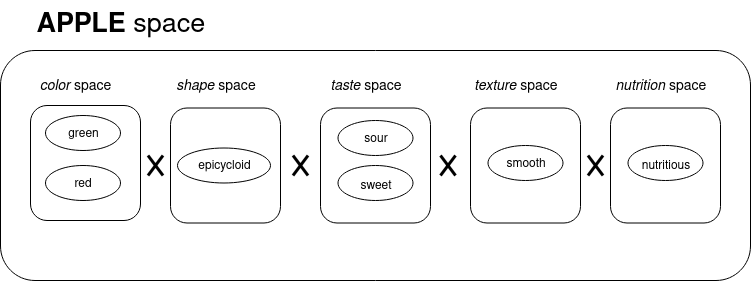
\includegraphics[width=\textwidth]{graphics/stolenfigures/apple_space.png}
	\slcaption{
		Inner form of a Conceptual Space for an apple, displayed as product of different properties, which are convex regions in different quality domain spaces. Reprinted from \cite{Hernandez-Conde2017}, who adapted it from \cite{Fiorini2013}.
	}
    \label{fig:apple_cs}
\end{figure}



\fbox{\begin{minipage}{40em}
    \newtheorem*{theorem*}{Conceptual Space}
    \begin{theorem*}
        A conceptual space is a geometric structure used to encode the meaning of natural language terms, properties and concepts. The metric space is spanned by \emph{quality dimensions} denoting basic domain-specific properties based on perception or sub-symbolic processing. Natural language categories (\emph{concepts}) correspond to convex regions, whereas points denote individual objects (instances/\emph{entities}, allowing for geometric solutions to commonsense reasoning tasks such as \emph{betweeness} or \emph{induction}.
        % \cite{Derrac2015}: "Conceptual spaces \cite{Gardenfors2000a} are metric spaces which are used to encode the meaning of natural language concepts and properties."
    \end{theorem*}
\end{minipage}}

Formally defined, a conceputal spaces needs the following definitions:
\begin{description}
    \item[Quality Dimensions] are atomic units of perception. Some of these are necessarily linked (such as hue and saturation), making them \textit{integral}, whereas others (\eg. temperature and weight) are \textit{seperable}. Typically each dimension corresponds to a primitive cognitive feature.
    \item[Domain] A set of integral dimensions that are seperable from others, like the \textit{color} domain made up from hue, saturation and value. Conceptual spaces are grouped into several low-dimensional subspaces according to these domains.
    \item[Similarity] is defined as inverse distance, which requries a metric. A distinction can be made for the aggregation of integral and separable dimensions. 
    \item[Betweenness] An object Y is between two other objects X and Z iff d(x,y) + d(y,z) = d(x,z).
    \item[Natural Properties (\textit{criterion P} \cite{Gardenfors2000a})] are defined as convex regions of a domain in a conceptual space. A convex region has the property that an interpolation between any two points in this region is necessarily also in this region. 
    \item[Concepts (\textit{criterion C} \cite{Gardenfors2000a})] are combinations of (potentially correlated) properties. \q{A concept is represented as a set of convex regions in a number of
    domains together with a prominence assignment to the domains and information about how the regions in different domains are correlated} \cite[8]{Gardenfors2004}
    \item[Entities] are specific instances (tokens) of a concept, encoded as points. 
    \item[Context] can be modelled in a CS by weighting certain dimensions higher than others, influencing distance and how concepts are fromed from properties.
\end{description}

Some corollaries: 

\begin{itemize}
    \item Each conceptual space contains only items for which the space's dimensions make sense, so you wouldn't find kings in a conceptual space of cabbages.
    \item Concepts roughly correspond to (non-proper) nouns, adjectives to properties and proper nouns (the name of a particular person, place, organization, or thing to points.)
    \item From the criterion of convexity for natural properties and the definition of betweenness, it follows that if an object Y is between X and Z, and both X and Z have a property, Y must also have this property.
    \item Relative properties can be defined as regions on a relative scale - the property "\textit{tall}" acccordingly can be defined to be true iff the entity is in the top 33\% \wrt the size-property of all relevant objects.
\end{itemize}

% \includeMD{pandoc_generated_latex/2_2_conceptualspaces}
\todoparagraph{look if I want to take a paragraph from 22conceptualspacesMD}
\todoparagraph{Rudiger had a formal definition in the CS course}

\subsection{Data-Driven Generation of Conceptual Spaces}

\includeMD{pandoc_generated_latex/2_3_datadrivengeneration}

\todoparagraph{Mit einem Satz (EINEM SATZ!!) erklaren dass wir den mit evaluaten werden indem wir gucken wie gut er dinge klassifizieren kann.}

\subsection{Explainable Reasoning with Conceptual Spaces}
% was "computational reasoning"
\label{sec:reasoning}

\todoparagraph{important for us is that we} don't have ONE SINGLE SIMILARTIY; BUT THAT IT's context-dependent!!!!

\todoparagraph{However a short paragraph about reasoning-based classifiers and the respective intutitive explanations for known classifiers}

The goal of this thesis is to provide explainable recommendation for educational resources. This section elaborates how the framework of \glspl{cs} allows to computationally model commonsense reasoning through analytic geometry and algebra.

\todoparagraph{We are looking how symbolistic stuff relates to CS}

According to \cite{Gardenfors2000a}, Representations don't need to be similiar to the objects they represent, but the *similarity relations of the representations* should correspond to those of the objects they represent

\subsubsection*{Categories and Ontologies}

% CS and with it ontologies "automatically" (BIG question mark) arise from prototypes + metric domain + voronoi tesselation

\todoparagraph{Vor allem sollte hier ruberkommen warum das gut fur mich und meinen recommender fur educational resources ist argh}

Logic-Based reasoning/inference can do many things already, however it requires the knowledge to be encoded in logic (a lot of manual work) and doesn't allow for fuzzyness.
In formal logic/ontologies/lexical databases, semantic relations of concepts are explicitly modelled. The \gls{rcc} \cite{Cohn1997a} links these relations to their geometric interpretation, providing a bridge between this and Conceptual Spaces \cite{Gardenfors2001}. Once you have created the structure, the following emerges automatically:

\vspace{2ex}

\begin{tabularx}{1.05\textwidth}{P{0.16\textwidth}|P{0.25\textwidth}|P{0.25\textwidth}|X}
    Ontology Relation & Other Names        & RCC5 \cite{Cohn1997a} analog / \textit{Geometric equivalent} & Example \\ \midrule

    Type Identity     & {\scriptsize Equality of Concepts, Synonymy } & Identical Regions (EQ)      & Animals with a liver \& Animals with a heart \\ 

    Subsumption       & {\scriptsize Hyponyms/ Hypernyms, \textit{is-a-relationship}, Concept Hierachies, Taxonomies }
                                           & Proper Parts(PP, PP\textsuperscript{-1}), \textit{Subregions}
                                                                          & \textit{Every pizzaria is a restaurant} \\  
    
    Mutual 
    Exclusiveness     &                    & Discrete Regions (DR), \textit{unconnected/disjoint regions}
                                                                          & \textit{No Restaurant can be a beach} \\  

    Overlapping 
    Concepts          &                    & Partial Overlap (PO)         & \textit{Some bars serve wine, but not all} \\  

    Opposites         &                    & \textit{Set inverse}         & Humans \& Non-human animals \\ 

    Token Identity    & {\scriptsize Equality of Names, Synonymy } & \textit{Equal coordinates}   & Morning star \& Venus \\ 
    Meronymy / Holonymy & {\scriptsize \textit{part-whole realationship} }& \textit{Product spaces} (see \cite{Fiorini2013}        & Trees \& Leaves
\end{tabularx}

regions and betweeness:
* convex hull as the set of all convex combinations of a point
* can be done by linear programming with polynomial cost


\vspace{4ex}

% Also: characteristics of properties (transitivity, symmetry) (from intrinsic features of dimensions (time is linear because the dimension is linear))

So for example the validity of "a robin is a bird" is encoded by it being a subregion. So, no reason for a symbolic inference when using the richer structure of CS instead of ontologies.

So a CS can model all semantic relations of classical ontologies/formal logic/symbolistic approaches/knowledge bases. However as it encodes more than just a taxonomy of concepts, it for higher/more forms of inference and (common-sense) reasoning, among others by enabling for interpolation and extrapolation of knowledge. These are:

\subsubsection*{Similarity-based reasoning}

\label{sec:similaritybasedreasoning}

As discussed already in \autoref{sec:amazonalgo}, modern recommendation algorithms often rely on similarity-based reasoning by suggesting that users that liked and item may also like similar items (collaborative filtering). In terms of classification, this corresponds to the 1-Neirest-Neighbor approach, where an object is assigned the class of the most similar item:\footnote{1-NN: \textit{Y is of the same class as X because X closest to Y}}

\noindent
\begin{minipage}{.6\textwidth}
  \syllogism{Alice likes \textit{the Lord of the Rings} \\
           \textit{The Hobbit} and \textit{Lord of the Rings} are similar}{Alice will probably like \textit{The Hobbit}}
\end{minipage}% 
\begin{minipage}{.4\textwidth}
  \syllogism{\textbf{A} has property \textbf{x} \\
             \textbf{B} is  similar to \textbf{A}}
             {\textbf{B} likely also has property \textbf{x}}
\end{minipage}% 

\vspace{2ex}

This is something that cannot be done by classical logic, which can not model degrees of something but only universal full truths. Another advantage is that it's easy to train, however a disadvantage is that it requires enough similar concepts which may not be given This algorithm however lacks \textit{explainability}: The employed distance function does not encode \textit{in what respect} two items are similar. For human reasoning however, there is no \textbf{overall Similarity} - instead similarity is relative to a domain and only meaningful in context \cite{Goodman1972-GOOPAP-3}: \q{any measurement of similarity is based on assumptions concerning the properties of a similarity relation} \cite[110]{Gardenfors2000a}. In a conceptual space, this can be modelled: The distance function can give weight for certain dimensions depending on context or objects of different concepts can be considered similar if they share enough properties. Most importantly however, in a CS a system for recommendation can ask users what dimensions of a given entity the user liked to suggest items that are similar in that regard.
% a system serving me a similar wine to the one I want that is not available can ask me what dimensions of that wine were important before suggesting new ones.

\subsubsection*{Induction}

Another very important tool of human common-sense reasoning is abstraction/generalization/ \textbf{induction}, going from single observations to general rules. For that, we need to decide which properties of the respective observation are relevant, distilling sensible information from the receptors from unimportant information to make inferences from limited information about an object? The connectionistic answer to that would be "pattern matching", and ML algorithms work extremely well for that, however this lacks explainability, and also we want to model the underlying algorithm and the underlying patterns. All three levels can model some kinds of induction and generalization, remember they are not in conflict. On the Conceptual Level you can eg model \textit{If two different entities of the same class have a property, maybe all entities of that class have a property}, which would be \textit{categroical inductive inverences}

\syllogism{Grizzly bears love onions \\
Polar bears love onions}
{All bears love onions \cite[226]{Gardenfors2000a}}

Other kinds of inductive reasoning we can model:

\textbf{Interpolative Reasoning}

\cite{Schockaert2011}: \q{intermediary conditions lead to intermediary conclusions} 

\noindent
\begin{minipage}{.6\textwidth}
  \syllogism{Cars have tires \\
             Bikes have tires \\
             Motorcycles are between cars and bikes
             }{Motorcycles likely also have tires}
\end{minipage}% 
\begin{minipage}{.4\textwidth}
    \syllogism{\textbf{A} has property \textbf{x} \\
               \textbf{C} has property \textbf{x} \\
               \textbf{B} is conceptually between \textbf{A} and \textbf{C}}
               {\textbf{B} likely also has property \textbf{x}}
\end{minipage}% 

% Source looking into it ([28] of [DESC15]): M. Abraham, D. Gabbay, U. Schild, Analysis of the talmudic argumen- tum a fortiori inference rule (kal vachomer) using matrix abduction, Studia Logica 92 (2009) 281–364.

\vspace{2ex}
\textbf{A fortiori reasoning}

\noindent
\begin{minipage}{.6\textwidth}
    \syllogism{\textit{The shining} is a horror film \\
            \textit{The shining} is scary \\
            \textit{It} is more scary than \textit{The shining}}
            {\phantom{penis} \\ 
            \textit{It} is likely also a horror film}
\end{minipage}% 
\begin{minipage}{.4\textwidth}
    \syllogism{\textbf{A} has property \textbf{x} \\
               \textbf{B} is \textit{more severe} than \textbf{A} \\ \phantom{penis}}
               {\textbf{B} likely also has property \textbf{x} \\ 
               \vspace{-0.5em} or a \textit{more severe} property}
\end{minipage}% 

\vspace{2ex}

\textbf{Extrapolative reasoning (Analogical Reasoning)} \cite{Schockaert2011}: \q{Analogous changes in the conditions should lead to analogous changes in the conclusion}, or \q{Concepts which differ in analogous ways have properties which differ in analaogous ways}. This is \textit{relational similarity}: If the analogical proportion a : b :: c : d holds, the pairs (a, b) and (c, d) are called relationally similar. Simply maps to geometric parallelism. 

I wrote down the syllogisms here, however that's not the only way to apply it, I can also "look for things that". In the case of analogies, I can ask "what is the thing that behaves to waterski like snowboarding to skiing"?

\textbf{Metaphors / Metonymy} (saying "the Pentagon" when referring to the US military) follow from a fortiori/analogical reasoning


\begin{figure}[H]
	\centering
	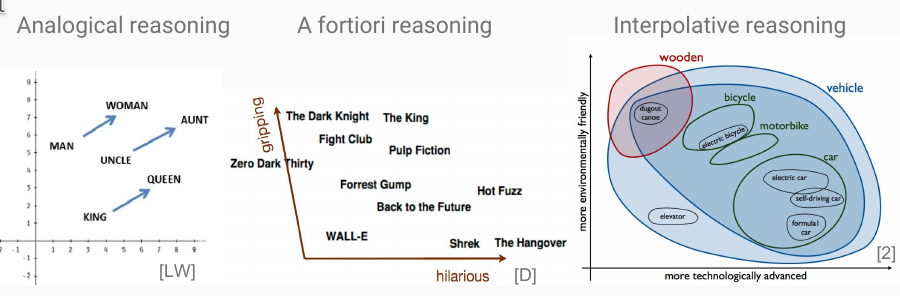
\includegraphics[width=\textwidth]{graphics/stolenfigures/reasoning_samples.png}
	\slcaption{
		Different forms of reasoning represented graphically. Holy shit remove me
	}
    \label{fig:graphic_reasoning}
\end{figure}

To automate these forms of inference, we need a richer form of knowledge than what is available in calssical logic: We need a notion of / Information about \textbf{Betweenness} and \textbf{Directionality}.

To model the stuff in \autocite{fig:graphic_reasoning}, we need a good metric, and what we see there definitely sounds euclidian!

\textbf{Summarized, CS are better than symbolism because we save the inference engine (plus we can extend and simulate knowledge bases with commonsense reasoning, just like humans deal with incomplete knowledge!) and better than connectionism because they are explainable. Klar soweit?!}

\todoparagraph{The problems of polysemy und synonymy for classical stuff, see fundamental information retrieval problem}


% \includeMD{pandoc_generated_latex/2_4_typesofreasoning}

\section{Other Related Work}
\label{sec:otherwork}

This thesis focuses on the aforementioned algorithm, primarily considering \cite{Derrac2015} and on top of that only two follow-up works: \cite{Ager2018, Alshaikh2020}, which have shown to provide useful extensions for it without changing its core logic. This shall by no means mean that these are the only ones that could be considered.

\paragraph{Tag Genome} 

By far the closest to what we do is the algorithm of \textcite{VISR12}, who generate a so-called tag genome for the domain of movies supervisedly based on keywords that users have assigned manually. Their algorithm takes these binary assignments and creates a dense representation that encodes a degree of relevance for each combination of movie and tag. Furthermore, they create a dedicated movie recommendation system on basis of this (interface reprinted in \autoref{fig:movietuner}). This system provides explainable recommendation based on these tags, allowing users to request recommendations for movies such as \textit{\q{I‘d like something less violent than Reservoir Dogs}} \cite[3]{VISR12}. Not only is their application exactly what is being demanded here, but the algorithm itself also performed significantly better than the one of \textcite{Derrac2015} in a human study of the latter, in which they directly compared the techniques by asking subjects which of the respectively extracted keywords better describes the difference between two movies \cite[44]{Derrac2015}. Considering however that \gencite{VISR12} algorithm is supervised and requires data which does not exist for our domain, it cannot be applied in our case. On the contrary, the final results of their algorithm are preferred by users over the ones generated with the algorithm considered in this work, but structurally exactly equal. This provides clear evidence that the desired application of this work is possible, albeit of lower quality than what their work achieved.

Generally, what is being done here corresponds to \textbf{Representation Learning}, whose aim is to discover the inherent semantic structure of a representation unsupervisedly \cite{Dayan1995}. More specifically \textbf{Disentangled Representation Learning}, where only salient attributes relevant to the task at hand should be extracted, which means finding latent embeddings whose dimensions are meaningful interpretable features. Generative Adversarial Networks \cite{Goodfellow2014} or Variational Autoencoders \cite{Kingma2013} are modern techniques that are good at finding latent information in images. Especially InfoGAN \cite{Chen2016} should be named, which can extract interpretable features such as pose, hairstyle, prensence of glasses and emotions from images unsupervisedly. 

\paragraph{LDA} 
\label{sec:lda}

In the realm of \gls{nlp}, this also relates to \textbf{Topic Modeling}, which aims to extract multiple hidden themes from a given text corpus by discovering groups of co-occuring words unsupervisedly. A well-known algorithm for this is Latent Dirichlet Allocation (LDA) \cite{Blei2003}, which represents documents by its salient \textit{topics}, each of which being a cluster of natural language terms. This technique bases on the assumption that each text consists of various topics, which are in turn made up by various keywords, making it possible to represent texts as multinomial distribution over latent topics which are aggregations of these keywords. Assuming a hierachical bayesian distribution where each text of a corpus is represented as mixture of topics it contains, their unsupervised algorithm extracts these by approximating the underlying infinite mixture of topic with an expectation-maximization (EM) algorithm. This yields a representation where each text is explicitly represented by the most propable words according to this distribution for a finite number of most probable topics. The algorithm finds use in text classification and collaborative filtering, but relies on unflexible \gls{bow} representations, making it hard to incorporate additional information such as correlations between topics \cite{Ager2018}.

\todoparagraph{LDA is still sometimes better than this algo} - see \autoref{tab:f1_mainalgos_me_short}


\paragraph{Academic Interests Recommender}
\label{sec:sidbert}
Regarding the used domain, there is already a system incorporated into the Siddata-\gls{dsa} that aids students by finding and recommending educational resources. SidBERT \cite{Schrumpf2021DELPHI} extracts implicit information from courses and other learning material by their title by categorizing them into one of 905 classes derived from the third or fourth level of the \gls{ddc} \cite{Dewey1876}, a hierachical tree stucture system commonly used to categorize library books. SidBERT uses the same dataset as this work and classifies with a custom classification head ontop of a \gls{bert}-encoder \gls{ann} which is trained on 1.3 million book titles collected from three universities as well as the German National Library, currently achieving 45.2\% test accuracy (62.2\% recall) among 905 classes.

\paragraph{Variations of this Algorithm}

There are also techniques that extend the algorithm of \textcite{Derrac2015}: \textit{Alshaikh et al.} \cite{Alshaikh2019, Alshaikh2021} use this algorithm as one of their steps and create a similar algorithm to find disentangled features, to be more in line with the original definition of Conceptual Spaces,which requires low-dimensional domain-specific subspaces. Regarding other unsupervised ways to create Conceptual Spaces, Peter Gärdenfors himself suggested in his book \cite{Gardenfors2000a} to use self-organizing maps (Kohonen-Networks \cite{Kohonen1997}) instead of classical \gls{nlp} algorithms and \gls{mds} to unsupervisedly create concpetual spaces. And finally, the whole concepts of vector-space models for words \cite{Mikolov2013} and texts \cite{Le2014,Devlin2019} is related in that represents the meaing of terms, phrases or documents by embedding them in a vector space. However these have arbitrary non-interpretable dimensions and are no metric spaces, thus having no relation of geometry and meaning for \eg betweeness or analogical reasoning, which will be eloborated in the next section.

\todoparagraph{BERT as best language model}


\section{Relevant Algorithms and Techniques}
\label{sec:required_algos}

\todoparagraph{dont forget the links for lsa und lda - are in lsa-long-md }

Thus far, we have described the base algorithm which this thesis replicates. Before describing each of its step in detail, it is useful to get a grasp of some general concepts relevant for it and its components. Furthermore, we will to put it into the context of the field of computational \gls{nlp} and elucidate some of the required theoretical foundation, and finally quickly look at what other techniques can be used for some of its components. \todoparagraph{Also, we need some general linear algebra bc after all these are vector spaces, so let's look quickly at projecting and playing around with coordinates}

\subsection{Classical Vector Space Construction}

\todoparagraph{Mention Distributional Hypothesis}

The algorithm consists of several steps/components, each of it of course is an algorithm in itself. The first steps are basically classical linguistic tools: Preprocessing \textrightarrow ~Bag-of-NGrams \textrightarrow ~Quantification \textrightarrow ~Frequency Matrix \textrightarrow ~Dimensionality Reduction (MDS) - followed by SVM-Classification\&Scoring \textrightarrow ~Clustering \textrightarrow ~Re-Embedding.

Many \gls{nlp} tasks rely on documents being represented as vectors, such as such as Information Retrieval, Recommendation, Text Classification, Translation, Sentiment Analysis among others \cite{Smith2017,bird2009natural,Devlin2019,Le2014,Mikolov2013a,Turney2010,Guo,Chen2018,Maas2011}. The process of turning a collection of texts document into numerical feature vectors is referred to as \textit{vectorization}. Let us explore some theoretical basis for that.

According to \textcite{Turney2010} (who in turn base their work on \textcite{Lowe}), the construction of a \gls{vsm} from texts can be decomposed into a four steps:\footnote{When considering neural embeddings such as \gls{word2vec}, the separation of these steps is hidden in the algorithm and not as distinct, but the principles hold also in these techniques.}

\begin{description}
    \item[1) Building the Frequency Matrix] which starts with preprocessing such as tokenization followed by normalizing and possibly \gls{lemma}tizing the tokens amongst many other possible techniques, before counting frequencies of either words or \glspl{ngram}, yielding a matrix of \glspl{bow}.
    \item[2) Transforming Raw Frequency Counts] \q{[B]ecause common words will have high frequencies, yet they are less informative than rare words} \cite{Turney2010}, it may make sense to adjust the weights of the elements of the frequency matrix.
    \item[3) Smoothing the Frequency Matrix] So far, the matrix is noisy, extremely sparse and extremely high-dimensional. Dimensionality Reduction helps to counter all three issues.
    \item[4) Calculating Similarities] of individual vectors as final step and aim of most algorithms. This can be done in various ways, a classical technique is to use the \gls{cos}.
\end{description}

Importantly, our algorithm differs from this four-step-process by injecting several additional steps before calculating similarities. This is because we hold the notion that similarity is necessarily context-dependent and there is no overall similarity (see \autoref{sec:reasoning}), which requires additional dissection of the final step.

Lets look at what all this means

\subsubsection{Bag-of-ngrams representation}
\label{sec:techniques:bow}

\includeMD{pandoc_generated_latex/2_bow}


\subsubsection{Word-weighting techniques}
\label{sec:word_count_techniques}

\todoparagraph{TODO: term? phrase? n-gram?}

When comparing the \gls{bow}-representations of texts, it is reasonable to give more weight to \emph{surprising} words than to expected ones. \q{The hypothesis is that surprising events, if shared by two vectors, are more discriminative of the similarity between the vectors than less surprising events.} \cite[156]{Turney2010} Another crucial reason is, that individual texts in the corpus are of drastically varying length, so longer entities would naturally dominate shorter ones when only comparing the raw counts - considering relative frequencies instead of absolute ones alleviates such problems. Because of these reasons, in the algorithm it will often be talked about \glspl{quant}. The algorithms explained below transforms the raw frequency-counts of a document and an \gls{ngram} into some \emph{score}, dependent on the number of occurences of this term in this document as well as the counts of other \glspl{ngram} and other documents. This score is henceforth called a \gls{quant}.

Let us consider term $t$, corpus $C$, document $d \in C$ (represented as \gls{bow}). Then:\\
term-frequency $\text{tf}_{t,d}$: How often $t$ occurs in $d$\\
document-frequency $\text{df}_t$: How many documents $\in C$ contain $t$\\
summed term-frequency $\text{df}_{t,*} = \sum_{d' \in C} \text{tf}_{t,d'}$: How often $t$ occurs in any document $\in C$

\paragraph{Tf-Idf} The most well-known technique formalizing this concept is the \gls{tf-idf}, which gives a term-document pair a higher weight if the term is generally rare in the corpus (low \textit{df}) and frequent in the respective document (high \textit{tf}):
\vspace{-3ex}
$$ w_{t,d} = \text{\textit{tf}}_{t,d} * log(\frac{|C|}{df_t}) $$

%see also: https://towardsdatascience.com/3-basic-approaches-in-bag-of-words-which-are-better-than-word-embeddings-c2cbc7398016
%\cite{Turney2010} (sec 4.2): Salton and Buckley (1988) defined a large family of tf-idf weighting functions and evaluated them on information re- trieval tasks, demonstrating that tf-idf weighting can yield significant improvements over raw frequency

\paragraph{PPMI}
% See also: https://stackoverflow.com/a/58725695/5122790

\textcite{Turney2010} suggested to use the \gls{ppmi} measure instead of \gls{tf-idf} to weight the counts in \glspl{doctermmat}, relying on \cite{Bullinaria2007}'s work taking into account psychological models to extract information about lexical semantics from co-occurence statistics. According to \cite{Turney2010,Bullinaria2007}, \gls{ppmi} performs most plausible to measure semantic similarity in word-context matrices compared to human evaluation. For that reason, \textcite{Derrac2015} and its follow-up works \cite{Ager2018,Alshaikh2020} rely solely on this technique. %(sec 4.2) of \cite{Turney2010}: Bullinaria and Levy (2007) demonstrated that PPMI performs better than a wide variety of other weighting approaches when measuring semantic similarity with word-context matrices.
Like tf-idf, it weights terms that are strongly associated with a document highly by favoring terms frequently associated with document $d$ while infrequent in the corpus overall. For that, it uses the \textit{log} of the probability of the term-document-combination, normalized by the probability of this $d$ with any $t$ and this $t$ with any $d$:
\vspace{-3ex}
\begin{align*}
   w_{t,d} &= max\left(0, log\left( \frac{p_{d,t}}{\sum_{t'}p_{d,t'}*\sum_{d'}p_{d',t}} \right) \right) \\
   p_{d,t} &= \frac{\text{tf}_{t,d}}{\sum_{d'}\sum_{t'} \text{tf}_{t',d'}}
\end{align*}

\todoparagraph{In practical terms}, efficient calculation of the PPMI-score for high-dimensional \glspl{doctermmat} requires excessives amounts of RAM, as it does not appear to be implemented in any major Python-library and its calculating requires multiplication of huge matrices.


\subsubsection{Dimensionality Reduction and Latent Space Embedding}
\label{sec:dim_red}

Next step is to smooth the frequency matrix. Goal is to keep comparison performance high, but make the  process faster and also ignore irrelevant noise \cite{Turney2010}.

We start with sparse vectors, and then \q{some form of dimensionality reduction is typically used to obtain vectors whose components correspond to concepts.} \cite{Derrac2015}


\paragraph*{LSA/LSA}

\textcite{Deerwester}

In fact, when using the right algorithms this has the additional effect to also find latent topics from tehse texts, which IMPOROVES similarity measurements bc now it's as if the latent stuff is in there

LSI relies on the \gls{distribhyp} in that it decomposes the matrix into the product of three matrices and then compresses them. Similar to AutoEncoders, if there is hidden information in the text than that will be used for this compression! 

\subsection{Other important Techniques}

includeMD{pandoc_generated_latex/2_othertechniques}








